
1 Introduction

2 ECAL Reconstruction Methods 
2.1 previous ( ratio ) method
2.2 Time Reconstruction - CC
2.2.1 Spike
2.2.2 Delay Times

3 ECAL Timing Performance
3.1 Performance Measurement
3.1.1 Resolution
3.1.2 Truth Times
3.1.3 Calibration
3.2 Performance of KUCC Algorithm in Data
3.3 Performance of KUCC Algorithm in Delayed Time MC 
3.4 Performance of KUCC Algorithm for Spike Rejection 

4 Summary 
5 References 




The arrival time of a pulse characterized by a rechit, or the rechit time, has a significant impact on the work done at the CMS experiment.  The rechit time allows us to differentiate information of interest seen by the detector from spurious background information.  Rechit times can also be used to determine the temporal location, and thereby the spatial location, of the originating interaction of the particle that generated the rechit.  This ability is central to many searches of physics beyond the standard model.  An example of of this will discussed in Section VIII.  In the case of OOT pile-up, the rechit time will be significantly before or after the nominal time for the current BX and by this criteria can be rejected from consideration.  Rechits can also be generated by particles that are the result of interactions with the material of the support structures for the detectors in CMS.  One particular issue of note in the ECAL is when a particle interacts with the photodetectors glued to the back of the crystals.  This gives rise to a spike that results in spurious rechits that do not arise from electromagnetic showers within the crystals.  Timing information is used to reject rechits coming from these spikes.  The resolution of the timing measurements made in the ECAL have a significant impact on the sensitivity of any analysis done in the CMS experiment.

\begin{figure}[htbp]
\begin{center}
\resizebox{0.48\linewidth}{!}{
\includegraphics{fig/sigma_Local_EBEB_Full_timefit_log_logx.pdf}}
\caption{Local resolution for Run 2017 miniAOD dataset.}
\label{timeresplot}
\end{center}
\end{figure}

\begin{figure}[htbp]
\begin{center}
\resizebox{0.48\linewidth}{!}{
\includegraphics{fig/timeres_gl2017.png}}
\caption{Time resolutions derived from the entirety of the Run 2017.  The resolution is shown for photons from $Z\rightarrow e^{+}e^{-}$, (\textit{Global}), and pairs of crystals in the same photon cluster, (\textit{Local}).  The \textit{Local} resolutions are further divided into crystal pairs in the same trigger tower, (\textit{Same}), and crystals pairs that are in different trigger towers, (\textit{Different}).  The category of Inclusive includes both \textit{Same} and \textit{Different} crystal pairs.}
\label{timeresgll}
\end{center}
\end{figure}

A complicating factor when determining time resolutions follows from consideration of the possibility that different back-end electronics were used to process the signals from the crystals.  If different electronics were used to process the signals from the two crystals in a selected crystal pair, this would have an impact on the time resolution.  In the ECAL, crystals are organized in groups that are referred to as trigger towers.  Each tower has separate back-end electronics to support the data taking and collection from the photodetectors on each trigger tower.  In many cases a pair of adjacent crystals from the same photon cluster will not be localized within the same trigger tower.  When this occurs the time resolution will be further degraded since we are then using two different sets of electronics to process the pulse information.  Time resolutions that are derived from crystal pairs within the same trigger tower are referred to as \textit{Local Same} resolutions.  Those derived from crystal pairs from adjacent trigger towers are referred to as \textit{Local Different} resolutions.  Time resolutions where the distinction between the \textit{Same} and \textit{Different} is not considered are referred to as \textit{Inclusive} resolutions.  All \textit{Global} resolutions are considered to be \textit{Global Inclusive}.

\begin{figure}[htbp]
\begin{center}
\resizebox{0.48\linewidth}{!}{
\includegraphics{fig/timeres_local_multisource.png}}
\caption{$Local Inclusive$ resolutions produced with miniAOD data samples are compared to resolutions produced with in-house reconstructions from raw datasets for Run 2016, 2017 and 2018.}
\label{timeresminraw}
\end{center}
\end{figure}

The time resolutions evaluated for all four cases, as shown in Figure~\ref{timeresgll}, demonstrate that the \textit{Local Inclusive} and \textit{Local Same} cases have the best resolution.  This is expected given that \textit{Local Same} resolutions are not degraded by the use of different back-end electronics and the majority of the crystal pairs for the \textit{Local} category will be in the same trigger tower.  The resolutions shown in Figure~\ref{timeresgll} were evaluated from datasets produced at CMS in which the reconstruction of the physics objects, like photons, is already completed.  These preprocessed datasets, provided in a data format called ``miniAOD'', discard much of the raw data collected in the experiment.  It was desirable for our work with the timing reconstruction, that will be discussed in Section VII, to have access to information that is only available in the raw data format.  A specialized platform was developed to reconstruct a limited set of physics objects from the raw datasets.  Figure~\ref{timeresminraw} compares the timing resolutions produced using miniAOD datasets and those produced using the specialized reconstruction from raw datasets.  As can be seen in this figure, the timing resolutions evaluated from the specialized reconstructions of the raw datasets is in good agreement with the resolutions evaluated from the miniAOD datasets.



In order to compare results from various timing algorithms it is necessary to preform the timing calibration for each of the algorithms.  Since it is not possible to run the official timing calibration on the algorithms under study, a calibration based on the average rechit time by channel was implemented.  For this calibration rechits where selected from reduced Egamma collection that have energies greater then 5 GeV.  To study the proposed timing algorithms, a rechit collection utilizing the timing algorithm to be studied was produced and time from the rechit that matched the selected rechit in the reduced Egamma collection is used in to create a calibration for that particular timing algorithm.

\begin{figure}[htbp]
\begin{center}
\resizebox{0.62\textwidth}{!}{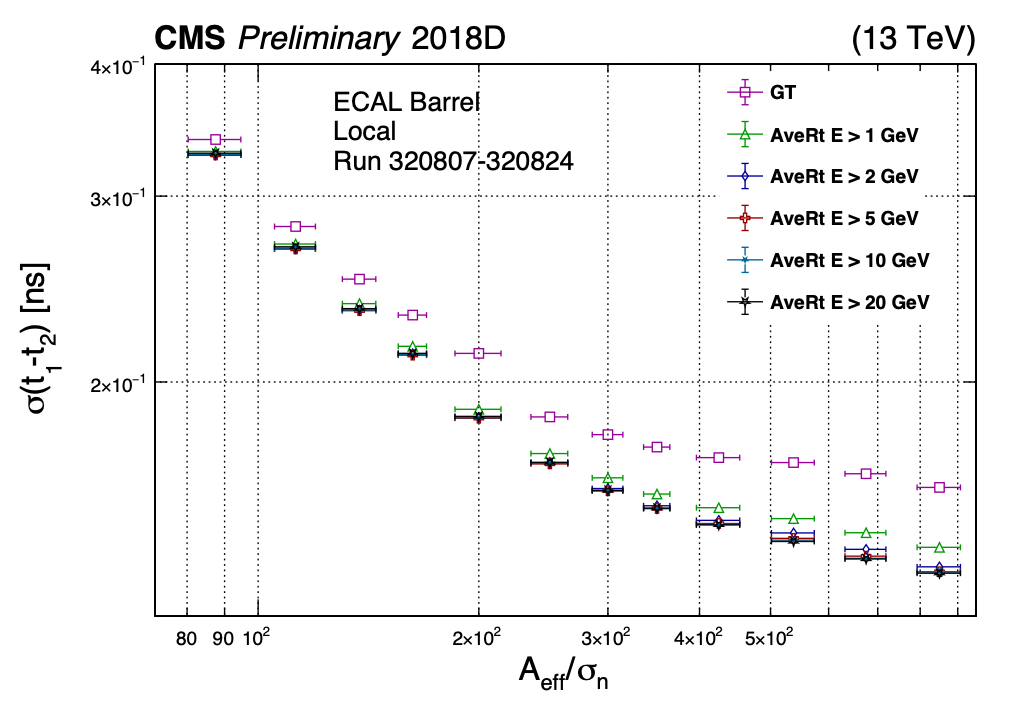
\includegraphics{fig/sec_method/e5cali.png}}
\caption{  ..  in-house calibration ...}
\label{e5cali}
\end{center}
\end{figure}




\begin{thebibliography}{99}
  
 %\cite{Bordry:2018gri} - done bordry2018machine
\bibitem{Bordry:2018gri} 
  F.~Bordry, M.~Benedikt, O.~Brüning, J.~Jowett, L.~Rossi, D.~Schulte, S.~Stapnes and F.~Zimmermann,
  ``Machine Parameters and Projected Luminosity Performance of Proposed Future Colliders at CERN,''
  arXiv:1810.13022 [physics.acc-ph].
  %%CITATION = ARXIV:1810.13022;%%
  %14 citations counted in INSPIRE as of 18 Sep 2019
  
%\cite{Evans:2008zzb} - done Evans:1129806
\bibitem{Evans:2008zzb} 
  L.~Evans and P.~Bryant,
  ``LHC Machine,''
  JINST {\bf 3}, S08001 (2008).
  doi:10.1088/1748-0221/3/08/S08001
  %%CITATION = doi:10.1088/1748-0221/3/08/S08001;%%
  %2507 citations counted in INSPIRE as of 13 Sep 2019
  
  %\cite{Chatrchyan:2008aa} - done Chatrchyan:1129810
  \bibitem{Chatrchyan:2008aa} 
    S.~Chatrchyan {\it et al.} [CMS Collaboration],
  ``The CMS Experiment at the CERN LHC.''
  JINST {\bf 3}, S08004 (2008).
  doi:10.1088/1748-0221/3/08/S08004
  %%CITATION = doi:10.1088/1748-0221/3/08/S08004;%%
  %6157 citations counted in INSPIRE as of 12 Sep 2019
  
    %\cite{Chatrchyan:2013lba} - done Chatrchyan_2013
\bibitem{Chatrchyan:2013lba} 
  S.~Chatrchyan {\it et al.} [CMS Collaboration],
  ``Observation of a New Boson with Mass Near 125 GeV in $pp$ Collisions at $\sqrt{s}$ = 7 and 8 TeV,''
  JHEP {\bf 1306}, 081 (2013)
  doi:10.1007/JHEP06(2013)081
  [arXiv:1303.4571 [hep-ex]].
  %%CITATION = doi:10.1007/JHEP06(2013)081;%%
  %768 citations counted in INSPIRE as of 13 Sep 2019
  
  %\cite{CMS:1997tlf} -= done Karimäki:368412
  \bibitem{CMS:1997tlf} 
  V.~Karimäki {\it et al.} [CMS Collaboration],
  ``The CMS tracker system project : Technical Design Report,''
  CERN-LHCC-98-006, CMS-TDR-5.
  %%CITATION = CERN-LHCC-98-006, CMS-TDR-5;%%
  %187 citations counted in INSPIRE as of 12 Sep 2019
  
%\cite{Tanabashi:2018oca} - done Tanabashi:2636832
\bibitem{Tanabashi:2018oca} 
  M.~Tanabashi {\it et al.} [Particle Data Group],
  ``Review of Particle Physics,''
  Phys.\ Rev.\ D {\bf 98}, no. 3, 030001 (2018) p. 448-462
  doi:10.1103/PhysRevD.98.030001
  %%CITATION = doi:10.1103/PhysRevD.98.030001;%%
  %2442 citations counted in INSPIRE as of 12 Sep 2019
  
  %\cite{Khachatryan:2015hwa} - done Khachatryan:1988091
\bibitem{Khachatryan:2015hwa} 
  V.~Khachatryan {\it et al.} [CMS Collaboration],
  ``Performance of Electron Reconstruction and Selection with the CMS Detector in Proton-Proton Collisions at $\sqrt{s}$ = 8  TeV,''
  JINST {\bf 10}, no. 06, P06005 (2015)
  doi:10.1088/1748-0221/10/06/P06005
  %[arXiv:1502.02701 [physics.ins-det]].
  %%CITATION = doi:10.1088/1748-0221/10/06/P06005;%%
  %684 citations counted in INSPIRE as of 12 Sep 2019
  
  %\cite{Adzic:2009aa} - done Adzic:1230325
\bibitem{Adzic:2009aa} 
  P.~Adzic {\it et al.} [CMS Collaboration],
  ``Radiation hardness qualification of PbWO(4) scintillation crystals for the CMS Electromagnetic Calorimeter,''
  JINST {\bf 5}, P03010 (2010)
  doi:10.1088/1748-0221/5/03/P03010
  [arXiv:0912.4300 [physics.ins-det]].
  %%CITATION = doi:10.1088/1748-0221/5/03/P03010;%%
  %29 citations counted in INSPIRE as of 12 Sep 2019
  
  %\cite{Anfreville:2007zz} - done ANFREVILLE2008292
\bibitem{Anfreville:2007zz} 
  M.~Anfreville {\it et al.},
  ``Laser monitoring system for the CMS lead tungstate crystal calorimeter,''
  Nucl.\ Instrum.\ Meth.\ A {\bf 594}, 292 (2008).
  doi:10.1016/j.nima.2008.01.104
  %%CITATION = doi:10.1016/j.nima.2008.01.104;%%
  %63 citations counted in INSPIRE as of 12 Sep 2019
  
  %\cite{Adzic:2007mi} - done Adzic:1009081
\bibitem{Adzic:2007mi} 
  P.~Adzic {\it et al.},
  ``Energy resolution of the barrel of the CMS electromagnetic calorimeter,''
  JINST {\bf 2}, P04004 (2007).
  doi:10.1088/1748-0221/2/04/P04004
  %%CITATION = doi:10.1088/1748-0221/2/04/P04004;%%
  %140 citations counted in INSPIRE as of 12 Sep 2019
    
  %\cite{CMS:2010ava} - done CMS-NOTE-2010-012
\bibitem{CMS:2010ava} 
  [CMS Collaboration],
  ``Electromagnetic calorimeter commissioning and first results with 7 TeV data,''
  CMS-NOTE-2010-012, CERN-CMS-NOTE-2010-012.
  %%CITATION = CMS-NOTE-2010-012, CERN-CMS-NOTE-2010-012;%%
  %45 citations counted in INSPIRE as of 13 Sep 2019
  
  %\cite{Massironi:2015yoa} - done massironi2015precision
\bibitem{Massironi:2015yoa} 
  A.~Massironi [CMS Collaboration],
  ``Precision electromagnetic calorimetry at the energy frontier: CMS ECAL at LHC Run 2,''
  arXiv:1510.02745 [physics.ins-det].
  %%CITATION = ARXIV:1510.02745;%%
  %1 citations counted in INSPIRE as of 13 Sep 2019
  
  %\cite{Chatrchyan:2009aj} - done Collaboration_2010
\bibitem{Chatrchyan:2009aj} 
  S.~Chatrchyan {\it et al.} [CMS Collaboration],
  ``Time Reconstruction and Performance of the CMS Electromagnetic Calorimeter,''
  JINST {\bf 5}, T03011 (2010)
  doi:10.1088/1748-0221/5/03/T03011
  [arXiv:0911.4044 [physics.ins-det]].
  %%CITATION = doi:10.1088/1748-0221/5/03/T03011;%%
  %45 citations counted in INSPIRE as of 13 Sep 2019
  
  %\cite{Chatrchyan:2013dga} - done CMS:2013lxn
\bibitem{Chatrchyan:2013dga} 
  S.~Chatrchyan {\it et al.} [CMS Collaboration],
  ``Energy Calibration and Resolution of the CMS Electromagnetic Calorimeter in $pp$ Collisions at $\sqrt{s} = 7$ TeV,''
  JINST {\bf 8}, P09009 (2013)
  [JINST {\bf 8}, 9009 (2013)]
  doi:10.1088/1748-0221/8/09/P09009
  [arXiv:1306.2016 [hep-ex]].
  %%CITATION = doi:10.1088/1748-0221/8/09/P09009;%%
  %271 citations counted in INSPIRE as of 13 Sep 2019
  
  %\cite{CMS:2019ulr} - doen CMS-PAS-EXO-19-005
\bibitem{CMS:2019ulr} 
  CMS Collaboration [CMS Collaboration],
  ``Search for long-lived particles using delayed photons with proton-proton collisions at $\sqrt{s}=13~\mathrm{TeV}$,''
  CMS-PAS-EXO-19-005.
  %%CITATION = CMS-PAS-EXO-19-005;%%
  
  %\cite{Khachatryan:2015iwa} - done CMS:2015myp
\bibitem{Khachatryan:2015iwa} 
  V.~Khachatryan {\it et al.} [CMS Collaboration],
  ``Performance of Photon Reconstruction and Identification with the CMS Detector in Proton-Proton Collisions at sqrt(s) = 8 TeV,''
  JINST {\bf 10}, no. 08, P08010 (2015)
  doi:10.1088/1748-0221/10/08/P08010
  [arXiv:1502.02702 [physics.ins-det]].
  %%CITATION = doi:10.1088/1748-0221/10/08/P08010;%%
  %291 citations counted in INSPIRE as of 13 Sep 2019
  
  %D. del Re, ?Timing performance of the CMS ECAL and prospects for the future?, J. Phys. Conf. Ser. 587 (2015), no. 1, 012003, doi:10.1088/1742-6596/587/1/012003.
  
  %\cite{ddelre:2015jpc} - done DelRe:1706325
\bibitem{ddelre:2015jpc}
  D. ~del Re, {\it et al.},
  ``Timing performance of the CMS ECAL and prospects for the future,''
  J.Phys.Conf.Ser. 587(2015), no. 01, 012003
  doi:10.1088/1742-6596/587/1/012003
  
  %\cite{Seiberg:1993vc} - done Seiberg_1993
\bibitem{Seiberg:1993vc} 
  N.~Seiberg,
  ``Naturalness versus supersymmetric nonrenormalization theorems,''
  Phys.\ Lett.\ B {\bf 318}, 469 (1993)
  doi:10.1016/0370-2693(93)91541-T
  [hep-ph/9309335].
  %%CITATION = doi:10.1016/0370-2693(93)91541-T;%%
  %460 citations counted in INSPIRE as of 14 Sep 2019
  
  %\cite{CMS:2015sjc} - done CMS-PAS-EXO-12-035
\bibitem{CMS:2015sjc} 
  CMS Collaboration [CMS Collaboration],
  ``Search for long-lived neutral particles in the final state of delayed photons and missing energy in proton-proton collisions at $\sqrt s$ = 8 TeV,''
  CMS-PAS-EXO-12-035.
  %%CITATION = CMS-PAS-EXO-12-035;%%
  %6 citations counted in INSPIRE as of 14 Sep 2019
 
 %\cite{DevParatma:2012qqa} - not found
\bibitem{DevParatma:2012qqa} 
  P.~S.~B.~Dev,
  ``Supersymmetric Inverse Seesaw and its Phenomenology,''
  %%CITATION = INSPIRE-1122592;%%
 
  %Rafael Teixeira de Lima and CMS Collaboration 2017 J. Phys.: Conf. Ser. 928 012005
  
\end{thebibliography}


\begin{center}
\begin{tabular}{ l }
\multicolumn{1}{c}{\Large HTo2LongLivedTo4b Monte Carlo Datasets}\\
\hline
\\
HTo2LongLivedTo4b\_MH-1000\_MFF-450\_CTau-100000mm\_TuneCP5\_14TeV-pythia8 \\
HTo2LongLivedTo4b\_MH-1000\_MFF-450\_CTau-10000mm\_TuneCP5\_14TeV-pythia8 \\
HTo2LongLivedTo4b\_MH-125\_MFF-12\_CTau-9000mm\_TuneCP5\_14TeV-pythia8 \\
HTo2LongLivedTo4b\_MH-125\_MFF-25\_CTau-15000mm\_TuneCP5\_14TeV-pythia8 \\
HTo2LongLivedTo4b\_MH-125\_MFF-25\_CTau-1500mm\_TuneCP5\_14TeV-pythia8 \\
HTo2LongLivedTo4b\_MH-125\_MFF-50\_CTau-30000mm\_TuneCP5\_14TeV-pythia8 \\
HTo2LongLivedTo4b\_MH-125\_MFF-50\_CTau-3000mm\_TuneCP5\_14TeV-pythia8 \\
HTo2LongLivedTo4b\_MH-250\_MFF-120\_CTau-10000mm\_TuneCP5\_14TeV-pythia8 \\
HTo2LongLivedTo4b\_MH-250\_MFF-120\_CTau-1000mm\_TuneCP5\_14TeV-pythia8 \\
HTo2LongLivedTo4b\_MH-250\_MFF-60\_CTau-10000mm\_TuneCP5\_14TeV-pythia8 \\
HTo2LongLivedTo4b\_MH-250\_MFF-60\_CTau-1000mm\_TuneCP5\_14TeV-pythia8 \\
HTo2LongLivedTo4b\_MH-250\_MFF-60\_CTau-500mm\_TuneCP5\_14TeV-pythia8 \\
HTo2LongLivedTo4b\_MH-350\_MFF-160\_CTau-10000mm\_TuneCP5\_14TeV-pythia8 \\
HTo2LongLivedTo4b\_MH-350\_MFF-160\_CTau-1000mm\_TuneCP5\_14TeV-pythia8 \\
HTo2LongLivedTo4b\_MH-350\_MFF-160\_CTau-500mm\_TuneCP5\_14TeV-pythia8 \\
HTo2LongLivedTo4b\_MH-350\_MFF-80\_CTau-10000mm\_TuneCP5\_14TeV-pythia8 \\
HTo2LongLivedTo4b\_MH-350\_MFF-80\_CTau-1000mm\_TuneCP5\_14TeV-pythia8 \\
HTo2LongLivedTo4b\_MH-350\_MFF-80\_CTau-500mm\_TuneCP5\_14TeV-pythia8 \\
%\\
%\hline
\label{mc_table}
\end{tabular}
\end{center}
